\subsection{Initial state}
Initially none of the transmission/reception latencies and asymmetry of White 
Rabbit devices or fiber parameters are known. Therefore {\bf the values of 
appropriate parameters should be set to 0 for all nodes and switches which will
be calibrated}. In the White Rabbit PTP Core this can be done by modifying the SFP
database and setting $\Delta_{TX}$, $\Delta_{RX}$ and $\alpha$ values to 0 for all
supported transceivers\footnote{Please refer to the White Rabbit PTP Core manual
\url{http://www.ohwr.org/projects/wr-cores/documents}}. For the White Rabbit Switch 
please modify the \emph{/wr/etc/sfp\_database.conf} and
\emph{/wr/etc/wrsw\_hal.conf} configuration files.

\subsection{Reference fiber latency}
\label{subsec:refiber}

In this very first step of the calibration procedure the total propagation delay
($\delta = \delta_{MS} + \delta_{SM}$) of a fiber cable is measured. It requires
two different fiber cables with LC connectors (i.e. fibers that have
different length). For further considerations let's mark them $f_1$ and $f_2$.
Fiber $f_1$ can be called helper and is just a few meters long. It is used to
measure the parameters of $f_2$ and in hardware calibration procedures described
later. Fiber $f_2$ is of the same type that will be used in the WR installation.
It is a few kilometers long and its parameters will be measured.

\begin{figure}[ht]
	\begin{center}
		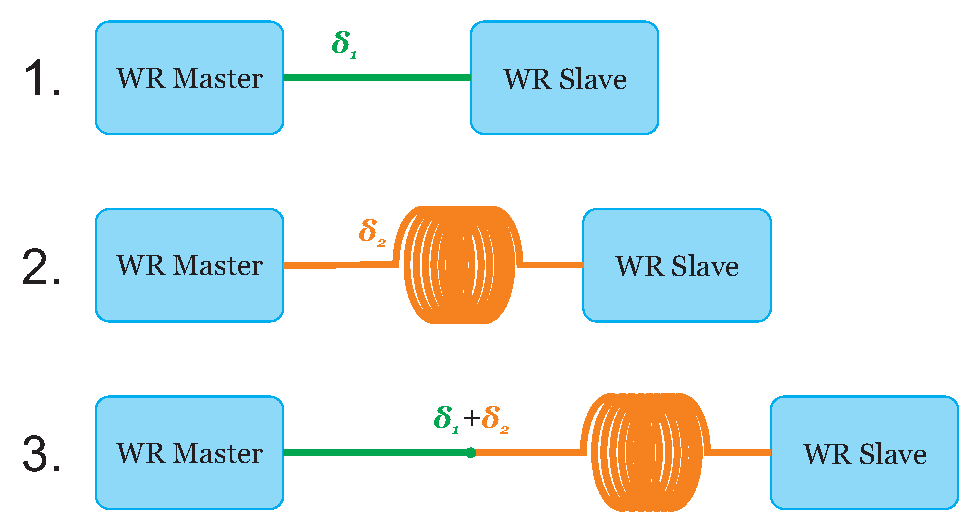
\includegraphics[width=.6\textwidth]{calibration/fiber_1.ps}
		\caption{Measuring total fiber propagation latency}
		\label{fig:refiber:latency}
	\end{center}
\end{figure}

\begin{enumerate}
	\item Take two White Rabbit devices, configure one of them as WR Master 
		and the other as WR Slave. 
	\item Connect them with fiber $f_1$ and wait until they become 
		synchronized (fig.\ref{fig:refiber:latency}, step 1). You can 
		use the available monitoring software \footnote{\emph{gui} WRPC 
		Shell command for the WR PTP Core, or \emph{wr\_mon} program for the WR 
		Switch} on the Slave device to check when it happens (indicated by 
		the WR servo in the \emph{TRACK\_PHASE} state and an offset below 1 ns).
	\item Write down the round trip delay ($delay_{MM1}$) reported by
		the monitoring software and the bitslide values for both
		Master($\epsilon_{M1}$) and Slave($\epsilon_{S1}$). Since the fixed delays
    are initially set to 0, the bitslide values are reported by the monitoring
		software simply as the reception delays.
	\item Connect the same two WR Devices with fiber $f_2$
		(fig.\ref{fig:refiber:latency}, step 2), wait again until the WR Slave
		becomes synchronized and write down the values of
		$delay_{MM2}$, $\epsilon_{M2}$ and $\epsilon_{S2}$.
	\item Connect fibers $f_1$ and $f_2$ together using an LC-LC Adapter and use
		this link to connect again the same WR Devices together(fig.
		\ref{fig:refiber:latency}, step 3). Wait until the WR Slave becomes 
		synchronized and write down the values of $delay_{MM3}$, 
		$\epsilon_{M3}$, $\epsilon_{S3}$.
	\item Subtract the bitslide values to obtain an approximation of the round
		trip delay, the sum of Master and Slave latencies ($\Delta_{TXM}$,
		$\Delta_{RXM}$, $\Delta_{TXS}$, $\Delta_{RXS}$) and the fiber round-trip
		latency:
		\begin{align}
			\label{equ:refiber:delmmeps1}
			delay_{MM1}' = delay_{MM1} - \epsilon_{M1} -
			\epsilon_{S1} \\
			\label{equ:refiber:delmmeps2}
			delay_{MM2}' = delay_{MM2} - \epsilon_{M2} -
			\epsilon_{S2} \\
			\label{equ:refiber:delmmeps3}
			delay_{MM3}' = delay_{MM3} - \epsilon_{M3} -
			\epsilon_{S3}
		\end{align}
	\item Calculate the latency of the fiber $f_1$ ($\delta_1$) and $f_2$
		($\delta_2$):
		\begin{align}
			\delta_1 = delay_{MM3}' - delay_{MM2}' \\
			\delta_2 = delay_{MM3}' - delay_{MM1}'
		\end{align}
		{\bf Note:} The LC-LC Adapter also has its own unknown latency that
		introduces an error in the $\delta_1$ and $\delta_2$ calculations.
		However, this error is a few picoseconds and can be disregarded.
\end{enumerate}
Further mathematical explanation for this calibration step can be found in
appendix \ref{subsec:app_filat}. Fiber cable $f_1$ with a round-trip latency
$\delta_1$ will be used further to pre-calibrate the selected WR Calibrator.

\subsection{Fiber asymmetry}
\label{subsec:fiasym}

The calibration of a fiber cable is needed to find out its asymmetry coefficient
$\alpha$. In the previous step we managed to calculate the total propagation
latency of fibers $f_1$ and $f_2$. However, to calibrate any device, the fiber
asymmetry has to be known.

The $\alpha$ coefficient used in the White Rabbit protocol to express fiber 
asymmetry is defined as:
\begin{equation}
	\alpha = \frac{\delta_{MS} - \delta_{SM}}{\delta_{SM}}
\end{equation}

To get its value, you have to make two connections with WR Devices and fibers
$f_1$, $f_2$ as presented in figure \ref{fig:fiasym}.

\begin{figure}[ht]
	\begin{center}
		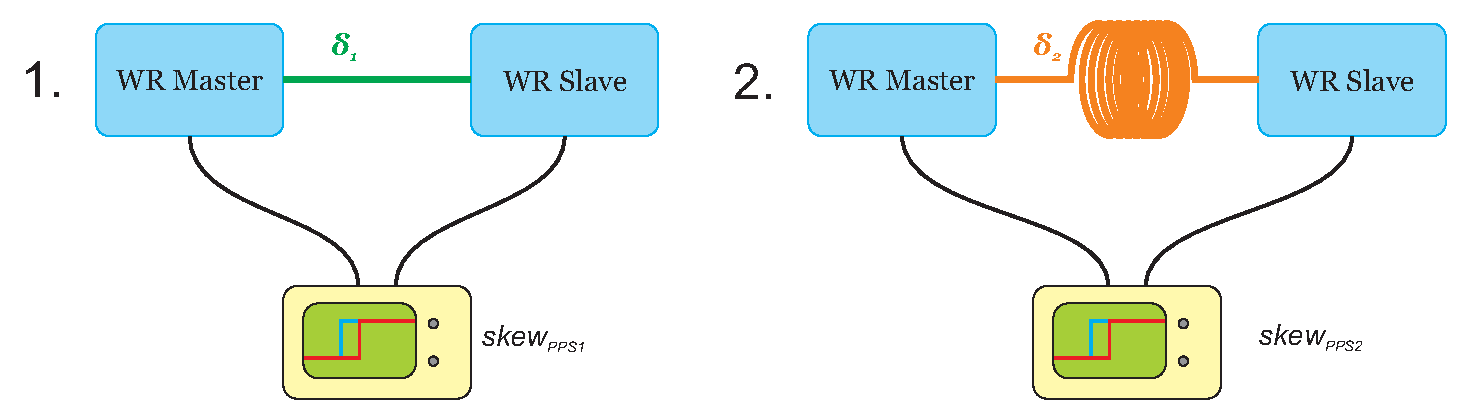
\includegraphics[width=.9\textwidth]{calibration/fiber_2.ps}
		\caption{Measuring fiber $f_2$ asymmetry}
		\label{fig:fiasym}
	\end{center}
\end{figure}

\begin{enumerate}
	\item Connect any two WR Devices with a few meters long fiber $f_1$, set
		the $\alpha$ value in their configuration to 0, configure one of them as WR
		Master, and the other as WR Slave. Connect their 1-PPS outputs to an
		oscilloscope. 
		
		It is important to use oscilloscope cables of the same length
		and type or cables with known delays so that no additional,
		unknown latency affects the measurements.

	\item Use the monitoring software to check when the Slave becomes
		synchronized to the Master (offset reported by WR PTP daemon below 
		1 ns and WR servo in the \emph{TRACK\_PHASE} state).

	\item Measure 1-PPS skew between the Slave and Master in picoseconds by
		comparing the 1-PPS signals with an oscilloscope ($skew_{PPS1} 
		= t_{PPS_S} - t_{PPS_M}$)

	\item Repeat the same procedure using a few kilometers long fiber $f_2$ to
		obtain the PPS skew for the second connection ($skew_{PPS2} =
		t_{PPS_S}' - t_{PPS_M}'$)

	\item Calculate the $\alpha$ coefficient using the following equation:
		\begin{equation}
			\alpha = \frac{2(skew_{PPS2} -
			skew_{PPS1})}{\frac{1}{2}\delta_2 -
			(skew_{PPS2}-skew_{PPS1})}
		\end{equation}

  \item The White Rabbit Switch uses the $\alpha$ value calculated from the equation
    above without any conversion. However, the White Rabbit PTP Core requires
    converting $\alpha$ into a natural number using the formula:
    \begin{equation}
      \alpha_N = 2^{40}(\frac{\alpha+1}{\alpha+2} - 0.5)
    \end{equation}

  \item $\alpha$ or $\alpha_N$ (depending on the WR Device) should be stored
		into the configuration parameters of a WR Calibrator but also into
		each Slave device that will use this fiber.
\end{enumerate}

Further mathematical explanation for this calibration step can be found in
appendix \ref{subsec:app_fiasym}

{\bf Note:} Both WR Devices used at CERN: the WR Switch and the WR PTP Core can
be used to calculate the $\alpha$ value. However, the 1-PPS signal generated by
the WR PTP Core running on the SPEC card with a DIO mezzanine is more jittery
than the 1-PPS generated by the WR Switch (check measurement uncertainty
considerations in appendix \ref{subsec:errors:fiasym}). For most applications
the inaccuracy of $\alpha$ measured using two SPEC cards will be negligible. If
that isn't the case, the most precise value of the $\alpha$ parameter can be
obtained from the measurements described above done with two WR Switches.
Alternatively, measurements done with two SPEC cards (or any other hardware
based on the SPEC design) can be repeated multiple times to produce an averaged
value of 1-PPS skew and a more accurate $\alpha$.


\subsection{Calibrator pre-calibration}
\label{sec:procedure:calibrator}

Having the parameters of fiber $f_1$ measured, a WR Calibrator has to be
selected among the set of available WR-compatible devices. The only
constraint for the selection is having two instances of the same device
for the pre-calibration procedure described here. They must have the
same PCB layout and the same FPGA bitstream.

To determine what are the transmission and reception latencies ($\Delta_{TX}$,
$\Delta_{RX}$) of the WR Calibrator, the connection shown in figure
\ref{fig:calibrator} has to be established.

\begin{figure}[ht]
	\begin{center}
		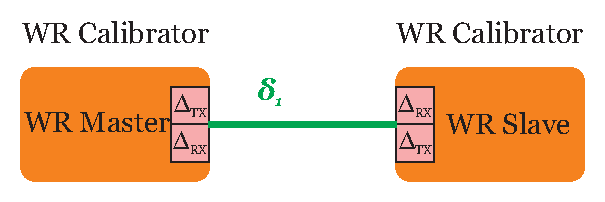
\includegraphics[width=.5\textwidth]{calibration/calibrator.ps}
		\caption{Measuring Calibrator latencies}
		\label{fig:calibrator}
	\end{center}
\end{figure}

\begin{enumerate}
	\item Since both Master and Slave are exactly the same devices (the same FPGA
		bitstreams, PCB layout, complementary SFPs from the same producer) the sum
		of their TX and RX latencies is equal:
		\begin{equation} 
			\Delta_{TXM} + \Delta_{RXM} = \Delta_{TXS} + \Delta_{RXS} 
		\end{equation}
		That means, the total transmission delay caused by each of those devices can
		be determined by simply dividing by 2 the round trip delay without the RX
		bitslide of each device and the fiber round-trip latency:
		\begin{equation}
			\Delta_{TX} + \Delta_{RX} = (delay_{MM1}' - \delta_1) /
			2
		\end{equation}
	\item Naturally, our Calibrator has some internal asymmetry, which means that
		$\Delta_{TX} \neq \Delta_{RX}$. There are two ways to determine the exact
		values of $\Delta_{TX}$ and $\Delta_{RX}$. It can be done either by
		establishing a WR link with a WR Device having a well-known internal
		asymmetry - which we don't have since all other devices will be calibrated
		from the WR Calibrator; or taking apart the Calibrator and measuring the
		latency of PCB traces, electronic components, SFP transceivers - that is
		possible, not trivial at all, and raises many other problems like measuring
		the latency between the SFP electrical input and its optical output, or
		measuring the latency inside the FPGA chip. Therefore at this point we set
		up a convention, that the WR Calibrator has no asymmetry:
		\begin{equation}
			\Delta_{TX} = \Delta_{RX}
		\end{equation}
		That means, the parameters describing the transmission and reception delays
		of the WR Calibrator should be set in the device configuration to:
		\begin{equation}
			\Delta_{TX} = \Delta_{RX} = (delay_{MM1}' - \delta_1) /
			4
		\end{equation}

		{\bf Note:} Don't worry, assuming that the WR Calibrator has no asymmetry
    does not affect the calibration quality. It is taken into account later
    during the actual calibration of each unknown WR Device. It also does not
    affect the WR PTP protocol when a link is established between two WR
    Calibrators, since the daemon only uses the precise value of the one-way,
    Master to Slave link delay (where the TX latency of the Master and RX
    latency of the Slave are summed together).
		
	\item Configure your WR Calibrator with the calculated $\Delta_{TX}$ and
		$\Delta_{RX}$ values - modify the SFP database for the WR PTP Core, or the
		\emph{/wr/etc/wrsw\_hal.conf} file for the WR Switch.
\end{enumerate}


\subsection{WR Device calibration} 
\label{subsec:devices}

Having the WR Calibrator selected among the available WR Devices, and the fiber
cable used in the previous steps (with known $\alpha$ coefficient and total
propagation delay $\delta$), you can start calibrating all other devices that
will later create a White Rabbit Network (fig.\ref{fig:devices}). 

\begin{figure}[ht]
	\begin{center}
		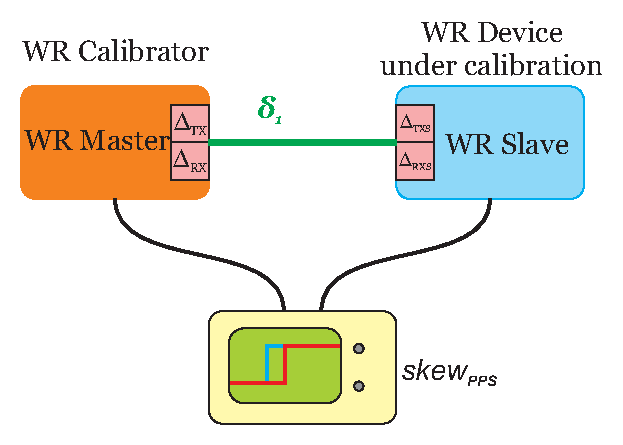
\includegraphics[width=.5\textwidth]{calibration/wr_device.ps}
		\caption{WR Device calibration with WR Calibrator and known
		fiber $f_1$}
		\label{fig:devices}
	\end{center}
\end{figure}

\begin{enumerate}
	\item Connect your Calibrator to an unknown WR Device using the fiber with the
		known $\alpha$ measured earlier (\ref{subsec:fiasym}). Remember to use an
		appropriate SFP transceiver on each side depending on whether your device
		under calibration is supposed to run as a WR Master or a WR
		Slave\footnote{There is a wiki page describing which wavelength should be
		used on each side: \url{http://www.ohwr.org/projects/white-rabbit/wiki/SFP}}.
		If you want to have the flexibility of selecting Master/Slave mode later
		through device configuration, the calibration procedure described below
		should be performed twice - with the SFP that will be used in Master, and
		the SFP that will be used in Slave mode. In further steps of this procedure
		the assumption is made that the WR Device being calibrated runs in WR Slave
		mode.
	\item Run the monitoring software on the Slave node and write down the
		round-trip delay ($delay_{MM}$) and fixed delays of both Master and Slave
		($\Delta_{TXM}$, $\Delta_{RXM}$, $\Delta_{TXS}$, $\Delta_{RXS}$). The
		transmission delay for Slave is reported to be 0, while the reception delay
		may be non-zero. It is the current RX bitslide value $\epsilon_S$.
	\item Calculate the average (coarse) transmission and reception delays for the
		Slave device:
		\begin{equation}
			\label{equ:devices:coarsedtxrx}
			\Delta_{TXS}' = \Delta_{RXS}' = \frac{1}{2} \Delta_S = 
			\frac{1}{2}(delay_{MM} - \Delta_{TXM} - \Delta_{RXM} - 
			\epsilon_S - \delta_1)
		\end{equation}
	\item Write the $\Delta_{TXS}$ and $\Delta_{RXS}$ delays to the configuration
		of your device, and restart its PTP daemon so that it synchronizes again
		using the new values.
	\item At this point your WR Device knows the coarse values of the transmission
		and reception delays. You can connect the 1-PPS signals generated by the
		calibrator and the device to an oscilloscope to observe that there is still
		some offset of (probably) a few nanoseconds between the Slave and Master
		even if the PTP daemon reports it is close to 0. That is because the
		transmission and reception delays are not equal (as the coarse values
		above). This asymmetry has to be measured and used to correct the coarse
		values of $\Delta_{TXS}$ and $\Delta_{RXS}$.
	\item Measure the Slave to Master offset by comparing the 1-PPS skew with the
		oscilloscope. This is the correction value that has to be subtracted from
		the coarse $\Delta_{TX}$ and added to $\Delta_{RX}$ to compensate the
		hardware asymmetry:
		\begin{align}
			\Delta_{TXS} = \frac{1}{2}\Delta_S - skew_{PPS} \\
			\Delta_{RXS} = \frac{1}{2}\Delta_S + skew_{PPS}
		\end{align}

		{\bf Note:} The asymmetry measured in this stage of calibration is in fact
		the sum of WR Device and WR Calibrator asymmetry. However, since both
		transmission and reception delays are modified with this value, the
		component for WR Calibrator asymmetry will cancel when connecting two WR
		Devices calibrated to the same Calibrator, see \ref{subsec:apx:devices} for
		a mathematical proof.
	\item After putting the new delay values in the configuration of the WR
		Device, the PTP daemon can be restarted and this time the device will
		synchronize to the Calibrator with an offset below 1ns.
	\item This procedure has to be repeated for all other WR Devices (WR Masters
		and WR Slaves). When you want to calibrate a WR Switch, this calibration
		procedure has to be performed for each WR port of the device.
\end{enumerate}
